\subsubsection{Plasma Treatment}
Exposing glass surfaces to plasma ---using a plasma cleaner--- 
has proven to be a crucial step to obtain 
high bonding energies. In 
the context of glass-to-glass bonding and many other applications, 
plasma (consisting of electrons, ions, free radicals, and 
photons) acts both as a cleaning and an activation agent  
\cite{rammhandbook, masteika2014, suniphd}.  
Figure~\ref{fig:plasma_act} illustrates some of the
many different processes that take place on the surface during 
plasma treatment; some of the most relevant ones are:
\begin{figure}[h]
\centering
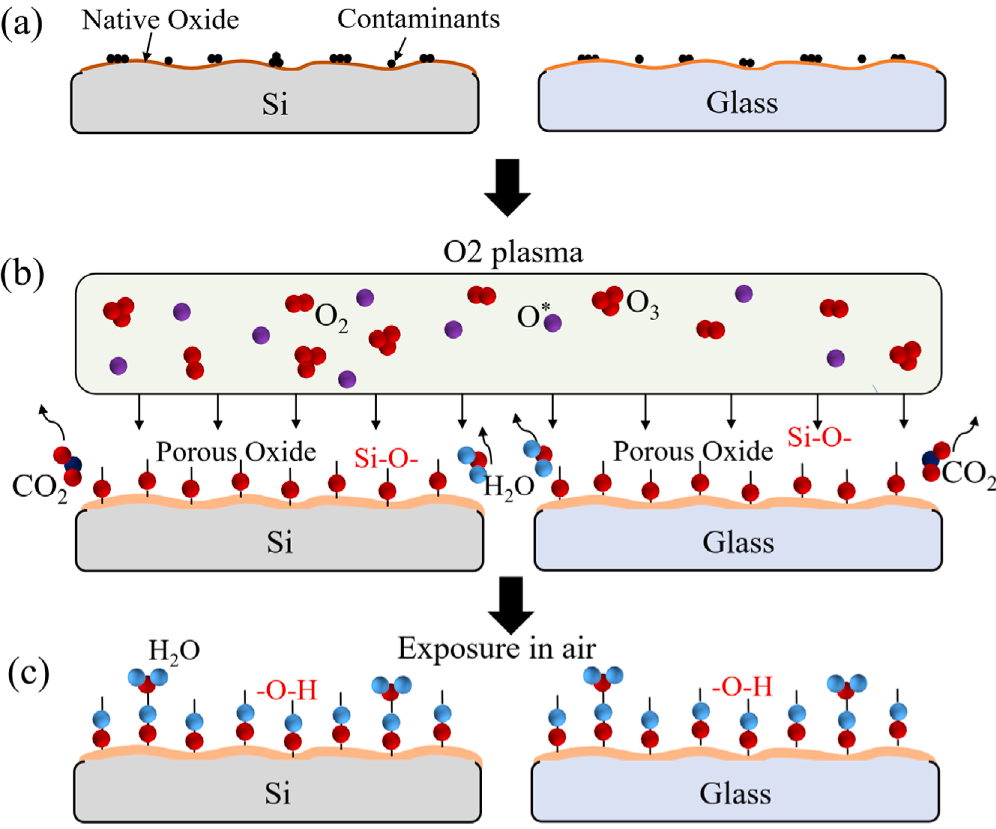
\includegraphics[width=0.75\linewidth]{Images/plasma_activation.png}
\caption{Effects of plasma treatment on silica surfaces. Plasma helps to remove 
    contaminants while increasing the number of available silanol groups.
    Adapted from \cite{yu2023}}
\label{fig:plasma_act}
\end{figure}
\begin{enumerate}
\item \textbf{Removal of contaminants from the surface:} Plasma removes contaminants from
    the surface ---specially organic matter--- and produces more dangling bonds,
    which leads to higher bonded areas.
\item \textbf{Increase in the number of silanol groups:} 
    Plasma initiates a modification of the surface,
     increasing its number of silanol groups (Si-O-), which are directly correlated to bonding strength.
\item \textbf{Improvement of the diffusivity of water and gas trapped at the interface:} 
    Plasma treatment increases diffusivity and thus enhances the evacuation of water and gas trapped 
    between the two glass substrates during the bonding stage. 
    Water evacuation is beneficial as it is needed to replace weak, 
    reversible hydrogen bonds ---which play a relevant role to start
    the bonding process--- by stronger Si-O-Si bonds. 
    Removal of trapped gas is also desirable, since it prevents the formation of bubbles during the annealing step.
\end{enumerate}
Common gases used in these plasma treatments are
$O_2$, $N_2$, and $Ar$. When operating a plasma cleaner,
 special attention must be paid to its power, chamber pressure, gas flow, and operating 
 times, as overexposure can lead to an increase of surface 
roughness and negatively affect the quality of the final bond.
\\\\
Exposing plasma-treated surfaces to chemicals should be avoided, since these 
substances have the capacity to etch or alter the surface,
effectively eliminating the benefits of this procedure \cite{neumann2021}. Therefore,
plasma treatment should be carried out after all chemical cleaning or activation steps.
Nevertheless, exposing plasma-treated surfaces to air or deionized water (DIW) has proven to be
beneficial, since water molecules can attach to the Si-O- groups present 
on the surface and create silanol (Si-OH) groups, which are crucial to start the bonding
process between two glass surfaces. Therefore, an effective workflow could be chemical 
cleaning and activation, followed by plasma treatment, a DIW rinse and finally
proceeding with pre-bonding and annealing.
\\\\
Plasma treatment becomes an essential tool in the context of low-temperature optical contact bonding, 
since it can yield 
strong bonding energies even at annealing temperatures as low 
as \SI{100}{\celsius} \cite{eichler2008}.
